\documentclass[main.tex]{subfiles}

\begin{document}

\section{Issue #2557}

When typing in Katex, Boostnote alignment doesn't work.

\subsection{Requirements}

This is a desktop software. Writing the following in edit panel:\\

\begin{verbatim}
$$
\begin{alignedat}{3}
    &P(X=x)={n \choose x}{m_1+\cdots+m_n\choose k}P^x(1-p)^{(n-x)}\\
    &E(X)=np\\
    &Var(X)=np(1-p)
\end{alignedat}
$$

And also

$$
\begin{array}{|c|c|c||c|c|c|}
    1 & 6 & 5 & 4 & 3 & 2
\end{array}
$$
\end{verbatim}

We get this result

\begin{figure}[h]
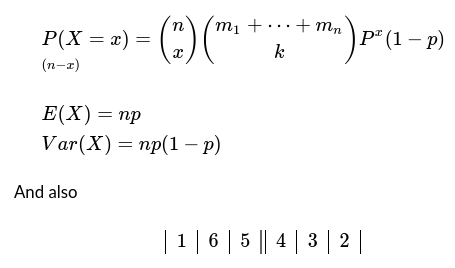
\includegraphics[scale=0.8]{images/bug.png}
\centering
\end{figure}
\clearpage

However, the expected result is

\begin{figure}[h]
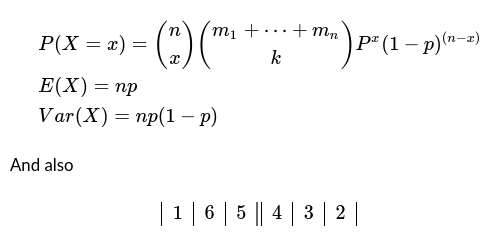
\includegraphics[scale=0.8]{images/result.png}
\centering
\end{figure}

The problem is that there is a linebreak where there should not be.

\subsection{Source Code Files}

The source code file that is involved with this issue is:

\begin{itemize}
\item  browser/components/markdown.styl
\end{itemize}

\subsection{System Architecture}

\subsection{Design of the fix}

There are two ways to fix this issue. At [katex.org](https://katex.org/) we check the list of styles applied to LaTeX shown on the front page and compared them to the CSS of Boostnote applied to the same LaTeX elements (display, text-align, white-space, and overflow-space). We concluded that the problem was in the tag white-space, whose value was normal through initial, instead of nowrap.\\

The initial value is applied to the body .katex selector whose priority is higher than the .katex selector, that defines white-space nowrap, which is the value expected.\\

The other possible solution is to change the selector used to have the same priority as the .katex selector.

\nocite{*}

\end{document}